\section{Specific Requirements}
\subsection{External Interface Requirements}
\subsubsection{User Interfaces}
The user interface of eMall is a mobile application, with an easy to use design.
It should be available on every major mobile operating system.
\subsubsection{Hardware Interfaces}
The system is fully operated on the Internet, so it doesn't feature any hardware interface, apart from the mobile device needed to access the service.
%\subsubsection{Software Interfaces}
\subsubsection{Communication Interfaces}
The main communication interfaces of the platform are the users and CPMSs.
The system interacts with users to receive booking requests or to send information, and to CPMSs to receive information about charging stations or to remotely interact with the charging socket.
A different interface is when the system sends push notifications to a user or retrieves the users' location, charging status and schedule.
%%% ==> CPMS
%%%
\subsection{Functional Requirements}

\subsubsection{Use case diagrams}
\begin{enumerate}
    \item \textbf{Unregistered Customer}
    \begin{figure}[H]
        \begin{center}
            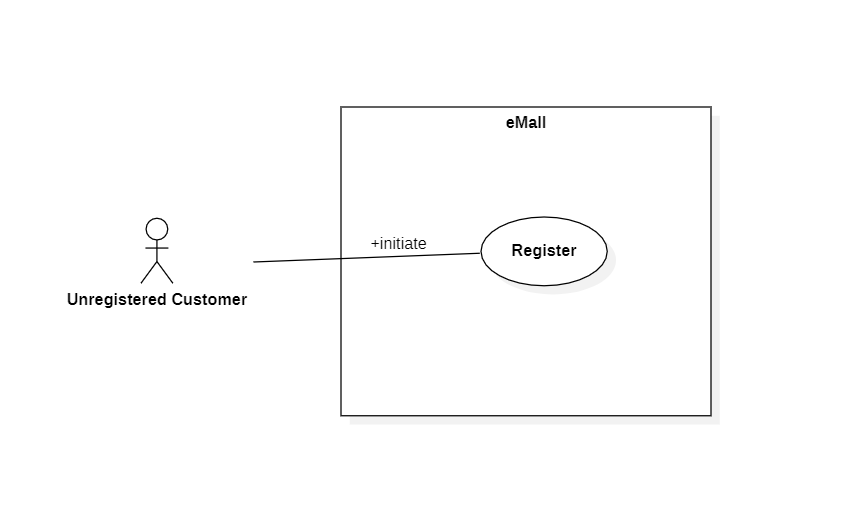
\includegraphics[width=\textwidth]{img/Unregistered_customer.PNG}
            \caption{Unregistered Customer - Use Case Diagram}
        \end{center}
    \end{figure}

    \item \textbf{Registered Customer}
    \begin{figure}[H]
        \begin{center}
            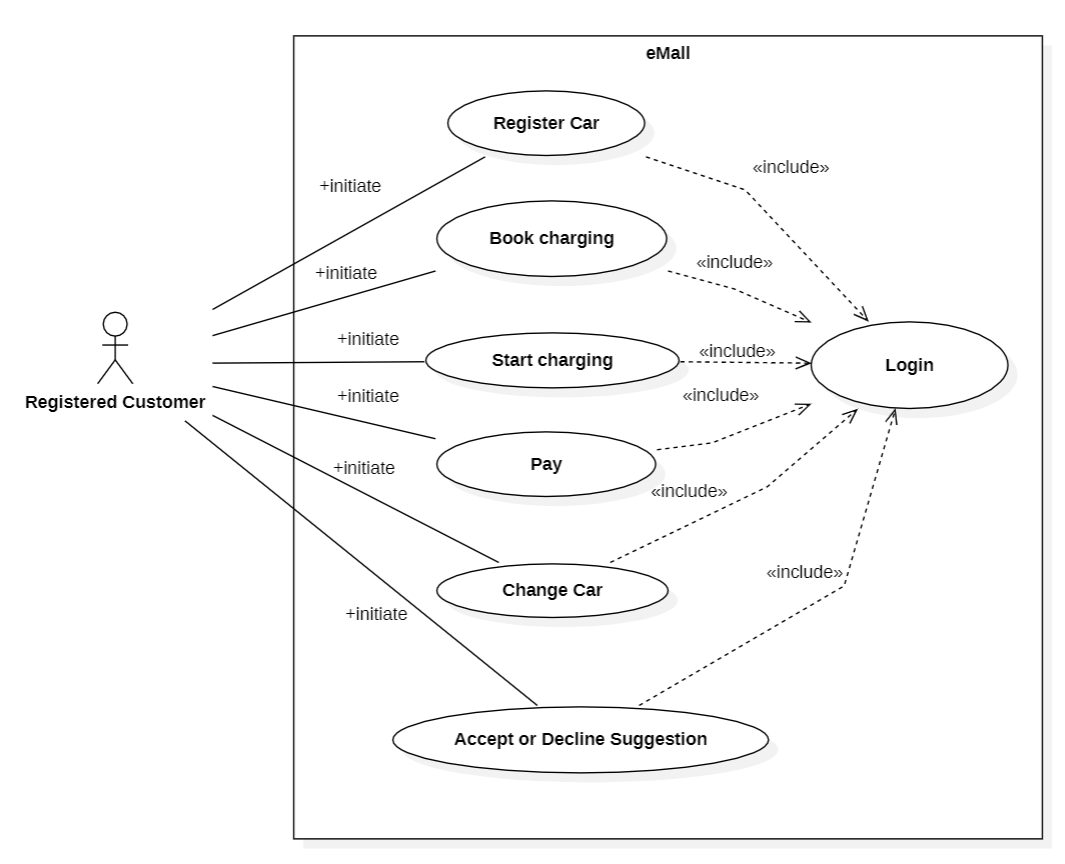
\includegraphics[width=\textwidth]{img/Registered_customer.PNG}
            \caption{Registered Customer - Use Case Diagram}
        \end{center}
    \end{figure}

    \item \textbf{Charging Point Operator}
    \begin{figure}[H]
        \begin{center}
            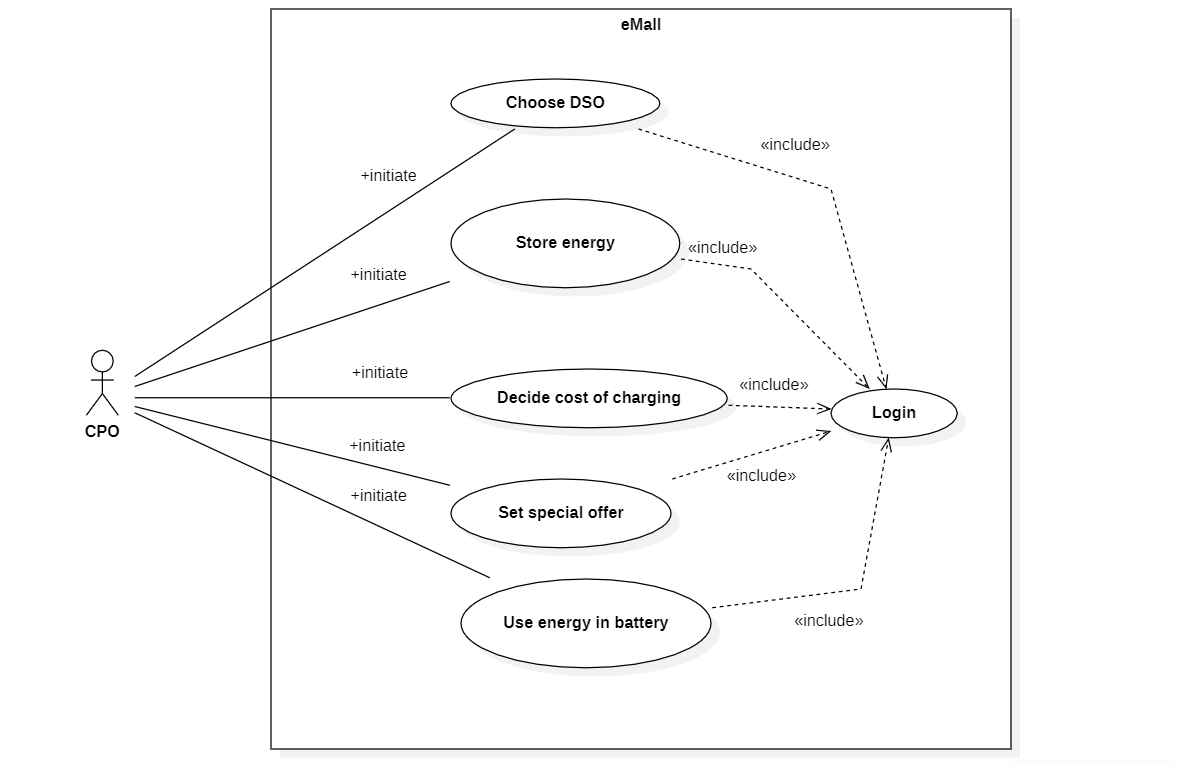
\includegraphics[width=\textwidth]{img/CPO_UseCase.PNG}
            \caption{Charging Point Operator - Use Case Diagram}
        \end{center}
    \end{figure}

\end{enumerate}
\subsubsection{Use case tables}
\subsubsection{Sequence diagrams}
This section shows all sequence diagrams related to the use cases. In all cases we consider that the actor has already logged in, except in the diagrams representing the registration and the login in operations.
\subsubsection{Requirements}
%TODO write requirements and map them with goals and domain assumptions
\subsubsection{Traceability Matrix}
%TODO mapping between requirements and use cases
\subsection{Performance Requirements}
\subsection{Design Constraints}
\subsubsection{Standards Compliance}
\subsubsection{Hardware Limitations}
\subsubsection{Any Other Constraint}

\subsection{Software System Attributes}
\subsubsection{Reliability}
The system must prevent downtime, in order to let Customers to charge their vehicle in every moment. At the same time CPO must be granted to access the system and perform their actions all the time.
To guarantee that the system is up most of the time, preventive regular maintanance should be perfomed. To make the system 24/07 accesible the server could be duplicated and the duplicated one run in parallel. So that during failures and maintanance, of one of them, users can access the other one.
\subsubsection{Availability}
Given the fact that eMall is not an emergency service or anything related to critical situations, the system must provide availability of 99.9\%. This means that the average time between the occurrence of a fault and service recovery (MTTR) has to be contained at around 0.365 days per year. 
\subsubsection{Security}
The data provided by the users contain some sensitive information, so the security aspect cannot be underestimated. The central database must be protected with all the available measures to avoid any external or internal attack. The passwords inside the data store have to be encrypted and in case of password recovery, this must never be sent in clear.
Communication between parties are encrypted and goes on a secure channel (through SSL protocol) to avoid traffic sniffing and spoofing, thus avoiding cheating attacks and guaranteeing privacy and consistency.
\subsubsection{Maintainability}
The system must guarantee a high level of maintainability. It must be designed in such a way that permits future addition of functionalities with minimum effort.
Design techniques must in fact guarantee an high reusability. The code must be well documented and hard-coding must be avoided. A testing routine has to be provided and it has to cover at least 75\% of the entire codebase, excluding interfaces code.


\subsubsection{Portability}
The application must be developed for two different platforms: iOS and Android smartphones. The web application must run on any OS (like Windows, Mac OS, Linux, etc) that supports a web browser. Even mobile devices like iPads and Android tablets must be able to access the web app.

